\ifdefined\ishandout
  \documentclass[handout,landscape]{beamer} 
\else
  \documentclass[landscape]{beamer}
\fi

%\hypersetup{pdfpagemode=FullScreen} %Enabling this option will cause the slides to go full-screen on opening

\mode<handout>
{
  \usepackage{pgf}
  \usepackage{pgfpages}

\pgfpagesdeclarelayout{6 on 1 boxed}
{
  \edef\pgfpageoptionheight{\the\paperheight} 
  \edef\pgfpageoptionwidth{\the\paperwidth}
  \edef\pgfpageoptionborder{0pt}
}
{
  \pgfpagesphysicalpageoptions
  {%
    logical pages=6,%
    physical height=\pgfpageoptionheight,%
    physical width=\pgfpageoptionwidth%
  }
  \pgfpageslogicalpageoptions{1}
  {%
    border code=\pgfsetlinewidth{1pt}\pgfstroke,%
    border shrink=\pgfpageoptionborder,%
    resized width=.5\pgfphysicalwidth,%
    resized height=.5\pgfphysicalheight,%
    center=\pgfpoint{.25\pgfphysicalwidth}{.833\pgfphysicalheight}%
  }%
  \pgfpageslogicalpageoptions{2}
  {%
    border code=\pgfsetlinewidth{1pt}\pgfstroke,%
    border shrink=\pgfpageoptionborder,%
    resized width=.5\pgfphysicalwidth,%
    resized height=.5\pgfphysicalheight,%
    center=\pgfpoint{.75\pgfphysicalwidth}{.833\pgfphysicalheight}%
  }%
  \pgfpageslogicalpageoptions{3}
  {%
    border code=\pgfsetlinewidth{1pt}\pgfstroke,%
    border shrink=\pgfpageoptionborder,%
    resized width=.5\pgfphysicalwidth,%
    resized height=.5\pgfphysicalheight,%
    center=\pgfpoint{.25\pgfphysicalwidth}{.5\pgfphysicalheight}%
  }%
  \pgfpageslogicalpageoptions{4}
  {%
    border code=\pgfsetlinewidth{1pt}\pgfstroke,%
    border shrink=\pgfpageoptionborder,%
    resized width=.5\pgfphysicalwidth,%
    resized height=.5\pgfphysicalheight,%
    center=\pgfpoint{.75\pgfphysicalwidth}{.5\pgfphysicalheight}%
  }%
  \pgfpageslogicalpageoptions{5}
  {%
    border code=\pgfsetlinewidth{1pt}\pgfstroke,%
    border shrink=\pgfpageoptionborder,%
    resized width=.5\pgfphysicalwidth,%
    resized height=.5\pgfphysicalheight,%
    center=\pgfpoint{.25\pgfphysicalwidth}{.167\pgfphysicalheight}%
  }%
  \pgfpageslogicalpageoptions{6}
  {%
    border code=\pgfsetlinewidth{1pt}\pgfstroke,%
    border shrink=\pgfpageoptionborder,%
    resized width=.5\pgfphysicalwidth,%
    resized height=.5\pgfphysicalheight,%
    center=\pgfpoint{.75\pgfphysicalwidth}{.167\pgfphysicalheight}%
  }%
}


  \pgfpagesuselayout{6 on 1 boxed}[letterpaper, border shrink=5mm]
  \nofiles
}

\usepackage{listings}
\usepackage{multimedia}
\usepackage[normalem]{ulem}
\usepackage{ifthen}
\usepackage{textcomp}

\usetheme{Warsaw} 
\usecolortheme{seahorse}
\useoutertheme{infolines} 

\setbeamertemplate{blocks}[rounded][shadow=true] 

\author{Joe Fields}
\title{Introduction to Proof} 

\date{Lecture 32 (GIAM \S 6.4) \newline ordering relations}
\institute[SCSU]{ {\tt fieldsj1@southernct.edu} }


\newlength{\cwidth}
\newcommand{\cents}{\settowidth{\cwidth}{c}%
\divide\cwidth by2
\advance\cwidth by-.1pt
c\kern-\cwidth
\vrule width .1pt depth.2ex height1.2ex
\kern\cwidth}

\newcommand{\sageprompt}{ {\tt sage$>$} }
\newcommand{\tab}{\rule{20pt}{0pt}}
\newcommand{\blnk}{\rule{1.5pt}{0pt}\rule{.4pt}{1.2pt}\rule{9pt}{.4pt}\rule{.4pt}{1.2pt}\rule{1.5pt}{0pt}}
\newcommand{\suchthat}{\; \rule[-3pt]{.25pt}{13pt} \;}
\newcommand{\divides}{\!\mid\!}
\newcommand{\tdiv}{\; \mbox{div} \;}
\newcommand{\restrict}[2]{#1 \,\rule[-4pt]{.125pt}{14pt}_{\,#2}}
\newcommand{\lcm}[2]{\mbox{lcm} (#1, #2)}
\renewcommand{\gcd}[2]{\mbox{gcd} (#1, #2)}
\newcommand{\Naturals}{{\mathbb N}}
\newcommand{\Integers}{{\mathbb Z}}
\newcommand{\Znoneg}{{\mathbb Z}^{\mbox{\tiny noneg}}}
\newcommand{\Enoneg}{{\mathbb E}^{\mbox{\tiny noneg}}}
\newcommand{\Qnoneg}{{\mathbb Q}^{\mbox{\tiny noneg}}}
\newcommand{\Rnoneg}{{\mathbb R}^{\mbox{\tiny noneg}}}
\newcommand{\Rationals}{{\mathbb Q}}
\newcommand{\Reals}{{\mathbb R}}
\newcommand{\Complexes}{{\mathbb C}}
%\newcommand{\F2}{{\mathbb F}_{2}}
\newcommand{\relQ}{\mbox{\textsf Q}}
\newcommand{\relR}{\mbox{\textsf R}}
\newcommand{\nrelR}{\mbox{\raisebox{1pt}{$\not$}\rule{1pt}{0pt}{\textsf R}}}
\newcommand{\relS}{\mbox{\textsf S}}
\newcommand{\relA}{\mbox{\textsf A}}
\newcommand{\Dom}[1]{\mbox{Dom}(#1)}
\newcommand{\Cod}[1]{\mbox{Cod}(#1)}
\newcommand{\Rng}[1]{\mbox{Rng}(#1)}

\DeclareMathOperator\caret{\raisebox{1ex}{$\scriptstyle\wedge$}}

\newtheorem*{defi}{Definition}
\newtheorem*{exer}{Exercise}
\newtheorem{thm}{Theorem}[section]
\newtheorem*{thm*}{Theorem}
\newtheorem{lem}[thm]{Lemma}
\newtheorem{cor}{Corollary}
\newtheorem{conj}{Conjecture}

\renewenvironment{proof}%
{\begin{quote} \emph{Proof:} }%
{\rule{0pt}{0pt} \newline \rule{0pt}{15pt} \hfill Q.E.D. \end{quote}}


\newcommand{\vs}{\rule{0pt}{11pt}}
\newcommand{\notimplies}{\;\not\!\!\!\implies}
\newcommand{\dx}{\,\mbox{d}x}

\AtBeginSection[]
{
 \begin{frame}{Table of Contents} 
  \tableofcontents[currentsection]
 \end{frame}
}

%%%% SAVE %%%%
%{ %magic to get a full screen image...
%\setbeamertemplate{navigation symbols}{}  % hide navigation buttons 
%\setbeamertemplate{background canvas}{\centerline{\includegraphics 
%	[height=\paperheight]{Cantor_4.jpeg}}}
%\begin{frame}[plain]
%\rule{0pt}{0pt}
%\end{frame} 
%} %end of magic


\begin{document}

\begin{frame}[plain]
  \titlepage
\end{frame}

\section{intro}

\begin{frame}{what is an ordering relation?}
\begin{itemize}
\item Total vs. partial orders.\pause
\item Comparability.\pause
\item Modeled after $\leq$ (except some things may not be comparable).
\end{itemize}
\end{frame}

\begin{frame}{the official definition}
\begin{itemize}
\item A relation $\relR$ on a set $S$ is an ordering relation if it is:\pause
\item Reflexive,\pause
\item Anti-symmetric,\pause
\item and Transitive.
\end{itemize}
\end{frame}

\begin{frame}{the other official definition}
\begin{itemize}
\item A relation $\relR$ on a set $S$ is a strict ordering relation if it is:\pause
\item Irreflexive,\pause
\item Anti-symmetric,\pause
\item and Transitive. \pause
\item These are also known as {\em irreflexive ordering relations} for obvious reasons.
\end{itemize}
\end{frame}

\begin{frame}{posets}
\begin{itemize}
\item Partially ordered sets -- posets \pause
\item A {\em poset} is a set $S$ together with a relation $\relR$ on $S$ that is an ordering relation\pause
\item Exercise 1 in Section 6.4 (on page 273 in GIAM).
\end{itemize}
\end{frame}


\begin{frame}{an example}
\begin{itemize}
\item My favorite ordering relation (after $\leq$) is the divisibility relation. \pause
\item (Note: this is not the strict sort.)\pause
\item Divisors of 12 (on page 267 in GIAM).
\end{itemize}
\end{frame}

\section{Hasse diagrams}

\begin{frame}{features}
\begin{itemize}
\item vertical position determines the direction\pause
\item drop all the loops\pause
\item don't show connections that can be deduced because of transitivity.
\end{itemize}
\end{frame}

\begin{frame}{examples}
\begin{itemize}
\item See pages 269 and 270 in GIAM.
\end{itemize}
\end{frame}

\begin{frame}{graded posets}
\begin{itemize}
\item Often one can find a function that determines the heights in a Hasse diagram.\pause
\item A graded poset consist of a set $S$, an ordering relation $\relR$ on $S$, and a function $\phi$ whose domain is $S$.\pause
\item If $x \neq y$ and $x \relR y$ then $\phi(x) < \phi(y)$ \pause
\item This property tells us that things that are mapped to the same value by $\phi$ can't be comparable.\pause
\item See the example on page 271
\end{itemize}
\end{frame}

\section{terminology}

\begin{frame}{chains and antichains}
\begin{itemize}
\item A \emph{chain} in a poset is a subset of the elements, all 
of which are comparable. \pause
\item An {\em antichain} in a poset is a subset
of the elements, none of which are comparable.\pause
\item Maximality -- A chain is {\em maximal} if it can't be added to. \pause
\item ditto for anti-chains.
\end{itemize}
\end{frame}

\begin{frame}{special elements}
\begin{itemize}
\item cover \pause (a.k.a. immediate successor) \pause
\item Maximality -- an {\em element} is maximal if it doesn't have a cover.\pause
\item An element is {\em minimal} if it doesn't cover anything.\pause
\item top/bottom \pause (a.k.a. greatest element and least element). \pause
\item This should remind you of relative and absolute maxima and minima. \pause
\item Exercise 2 in Section 6.4.
\end{itemize}
\end{frame}

\begin{frame}{hypercubes}
\begin{itemize}
\item The power set of a set partially ordered by $\subseteq$ \pause
\item This is a graded poset with $\phi(A) = |A|$.
\item Let's draw a few.
\end{itemize}
\end{frame}

\begin{frame}{\sout{hyper}cubes}

\begin{picture}(0,0)%
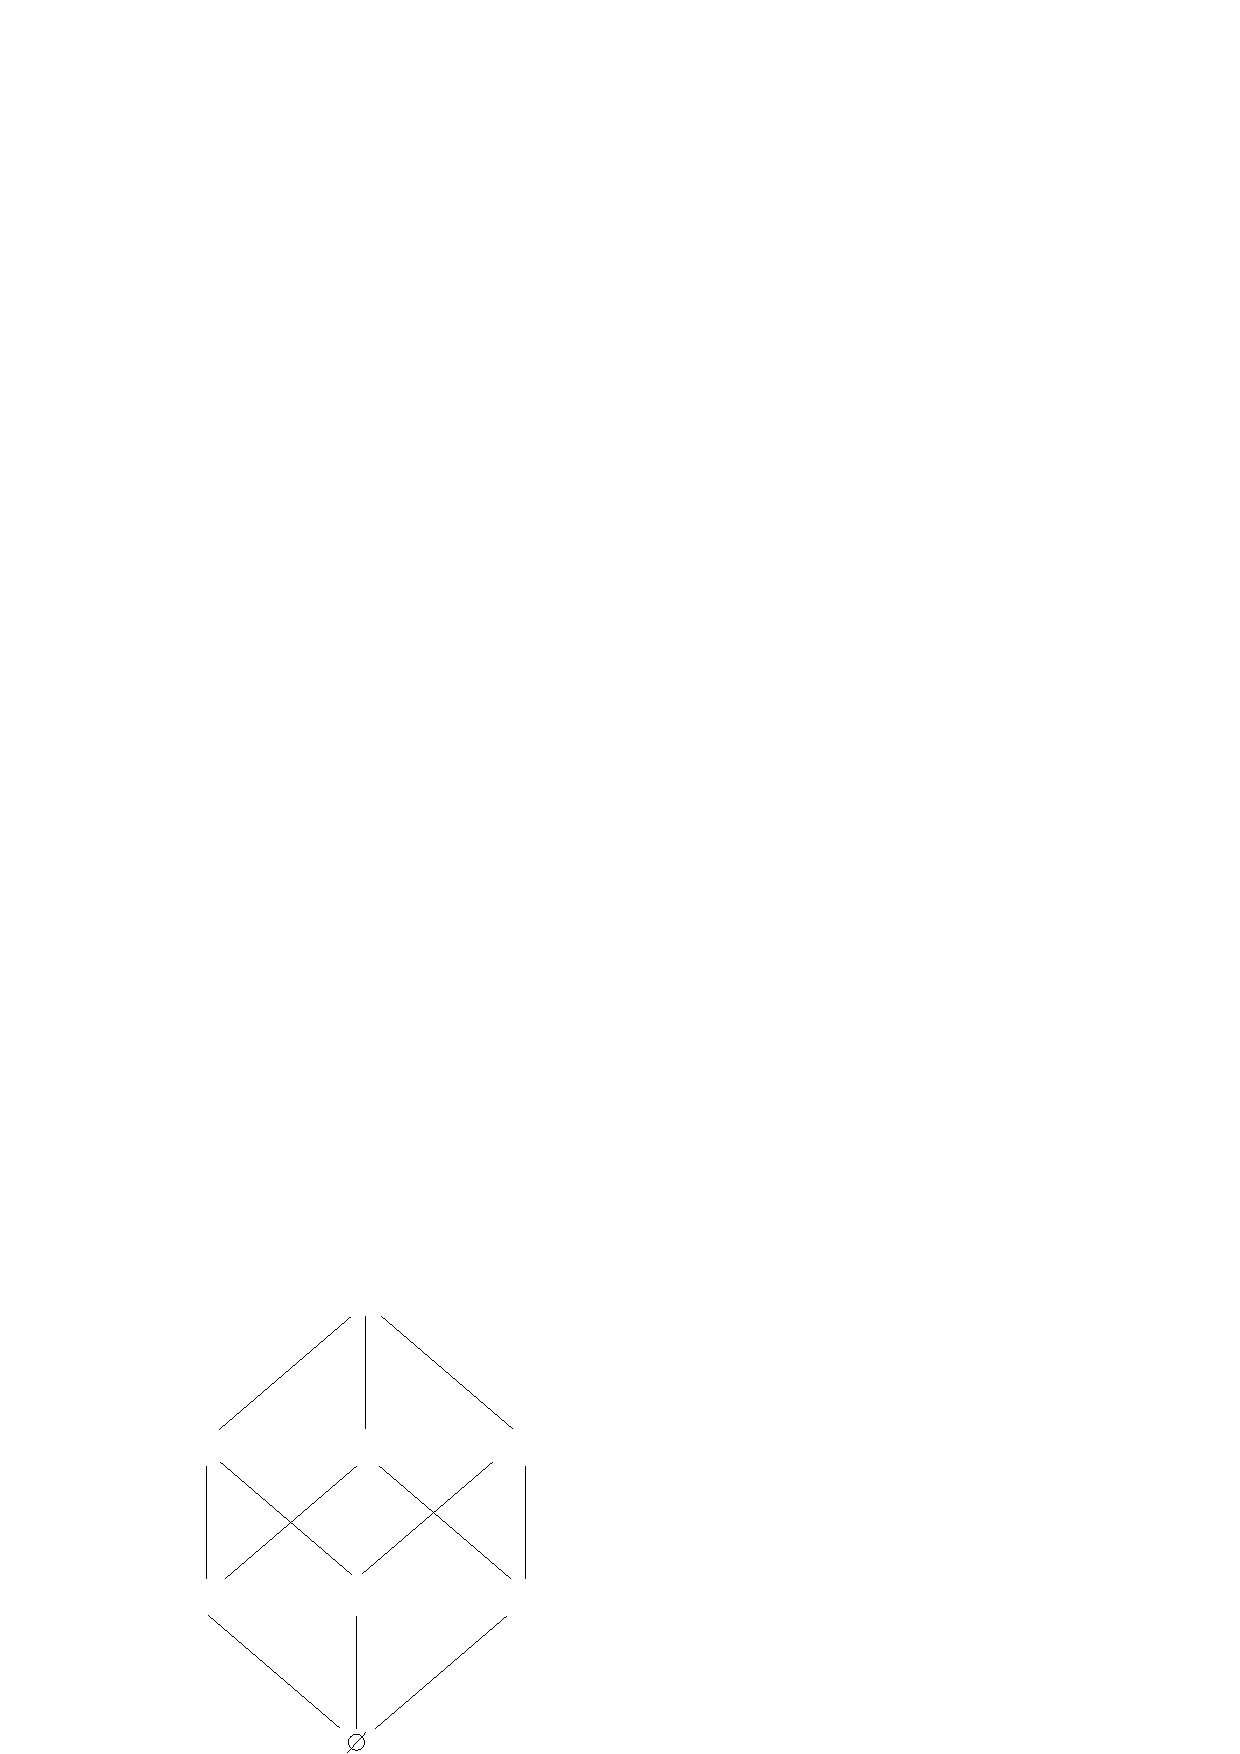
\includegraphics{figures/Hasse_for_subsets.pdf}%
\end{picture}%
\setlength{\unitlength}{3947sp}%
%
\begingroup\makeatletter\ifx\SetFigFont\undefined%
\gdef\SetFigFont#1#2#3#4#5{%
  \reset@font\fontsize{#1}{#2pt}%
  \fontfamily{#3}\fontseries{#4}\fontshape{#5}%
  \selectfont}%
\fi\endgroup%
\begin{picture}(4213,3724)(3300,-3938)
\put(4801,-2761){\makebox(0,0)[lb]{\smash{{\SetFigFont{12}{14.4}{\rmdefault}{\mddefault}{\updefault}{\color[rgb]{0,0,0}$\{1\}$}%
}}}}
\put(6001,-2761){\makebox(0,0)[lb]{\smash{{\SetFigFont{12}{14.4}{\rmdefault}{\mddefault}{\updefault}{\color[rgb]{0,0,0}$\{2\}$}%
}}}}
\put(7201,-2761){\makebox(0,0)[lb]{\smash{{\SetFigFont{12}{14.4}{\rmdefault}{\mddefault}{\updefault}{\color[rgb]{0,0,0}$\{3\}$}%
}}}}
\put(7126,-1561){\makebox(0,0)[lb]{\smash{{\SetFigFont{12}{14.4}{\rmdefault}{\mddefault}{\updefault}{\color[rgb]{0,0,0}$\{2,3\}$}%
}}}}
\put(5926,-1561){\makebox(0,0)[lb]{\smash{{\SetFigFont{12}{14.4}{\rmdefault}{\mddefault}{\updefault}{\color[rgb]{0,0,0}$\{1,3\}$}%
}}}}
\put(4726,-1561){\makebox(0,0)[lb]{\smash{{\SetFigFont{12}{14.4}{\rmdefault}{\mddefault}{\updefault}{\color[rgb]{0,0,0}$\{1,2\}$}%
}}}}
\put(5851,-361){\makebox(0,0)[lb]{\smash{{\SetFigFont{12}{14.4}{\rmdefault}{\mddefault}{\updefault}{\color[rgb]{0,0,0}$\{1,2,3\}$}%
}}}}
\end{picture}%


\end{frame}


{ %magic to get a full screen image...
\setbeamertemplate{navigation symbols}{}  % hide navigation buttons 
\setbeamertemplate{background canvas}{\centerline{\includegraphics 
 [height=\paperheight]{4-cube.png}}}
\begin{frame}[plain]
\rule{0pt}{0pt}
\end{frame} 
} %end of magic


\end{document}
